\documentclass{article}
\title{Perceptron and Neural Networks}
\author{Huang Yanzhen}

\setlength{\parskip}{0.5em}%
\setlength{\parindent}{0pt}%

\usepackage{amssymb}
\usepackage{amsmath}
\usepackage{algorithm2e}
\usepackage{tikz}
\usetikzlibrary{positioning}

\begin{document}
\maketitle
\section{Perceptron Algorithm}
\subsection{Problem Setup}\label{ssection:problem-setup}

\textbf{Given:}

A set of $l$-dimensional data samples:

\begin{equation}
    \mathcal{X} = \{\mathbf{x}_{1}, \mathbf{x}_2, \ldots, \mathbf{x}_{N}\} \subset \mathbb{R}^{l}
\end{equation}

Two classes:

\begin{equation}
    \Omega = \{\omega_{1}, \omega_{2}\}
\end{equation}

A ground-truth classification relation (i.e., which sample belongs to which class):

\begin{equation}
    R: \mathcal{X} \mapsto \Omega
\end{equation}

\textbf{Do:}

Our goal is to decide a hyperplane $g(\mathbf{x})$:

\begin{equation}
    g(\mathbf{x}): \mathbf{w}^\top \mathbf{x} + w_{0} = 0
\end{equation}

where $\mathbf{w}$ is the $l$-dimensional column weight vector and $w_{0}$ 
is the threshold. 

Assume that the classes are linearly seperable. Thus, we 
are able to find a weight vector $\mathbf{w}$ that separates the two types.

\begin{equation}
    \exists \mathbf{w}, w_{0}, \ 
    \begin{cases}
        \mathbf{w}^\top \mathbf{x} + w_{0} > 0, \ R(\mathbf{x}) = \omega_{1} \\
        \mathbf{w}^\top \mathbf{x} + w_{0} < 0, \ R(\mathbf{x}) = \omega_{2}
    \end{cases}
\end{equation}

\subsection{Notations}

More specifically, we can write the hyperplane as:

\begin{equation}
    g(\mathbf{x}): 
    \begin{bmatrix}
        w_{1} & w_{2} & \cdots & w_{l}
    \end{bmatrix}
    \cdot
    \begin{bmatrix}
        x_{1} \\ x_{2} \\ \vdots \\ x_{l}
    \end{bmatrix}
    + w_{0} = 0
\end{equation}

This is equivalent to:

\begin{equation}
    g(\mathbf{x}): 
    \begin{bmatrix}
        w_{1} & w_{2} & \cdots & w_{l} & w_{0}
    \end{bmatrix}
    \cdot
    \begin{bmatrix}
        x_{1} \\ x_{2} \\ \vdots \\ x_{l} \\ 1
    \end{bmatrix}
    = 0
\end{equation}

To unify everything into matrix calculation, we omit the explicit
expression of the threshold $w_{0}$ by:

\begin{align}
    \mathbf{w}_{\text{new}} = \begin{bmatrix}
        \mathbf{w}_{\text{old}} \\ w_{0}
    \end{bmatrix} \\
    \mathbf{x}_{\text{new}} = \begin{bmatrix}
        \mathbf{x}_{\text{old}} \\ 1
    \end{bmatrix}
\end{align}

Namely,
\begin{equation}
    \mathbf{w}_{\text{old}}\mathbf{x}_{\text{old}} + w_{0} 
    \equiv \mathbf{w}_{\text{new}} \mathbf{x}_{\text{new}}
\end{equation}

The property of the hyperplane  mentioned in 
\ref{ssection:problem-setup} would be written as follows:

\begin{equation}
    \exists \mathbf{w} \in \mathbb{R}^{l+1}, 
    \begin{cases}
        \mathbf{w}^\top \mathbf{x} > 0 & R(\mathbf{x}) = \omega_{1} \\
        \mathbf{w}^\top \mathbf{x} < 0 & R(\mathbf{x}) = \omega_{2} \\
    \end{cases}
\end{equation}

In the following part of the document, this notation is implicitly used.

\clearpage

\subsection{Perceptron and Hyperplane}
\begin{description}
    \item[Definition] A perceptron represents a smart hyperplane. 
\end{description}

Suppose we have a set of numerical input $\mathbf{x}=\begin{bmatrix}
    x_{1} & x_{2} & \cdots & x_{l} & 1
\end{bmatrix}^\top$. A perceptron has:
\begin{itemize}
    \item An adder weights $\mathbf{w} \in \mathbb{R}^{l+1}$ that sums the input.
    \item A smart decision unit $f$ called \textbf{activation function} that activates the sum result by the adder.
\end{itemize}

\begin{figure}[h]
    \centering
    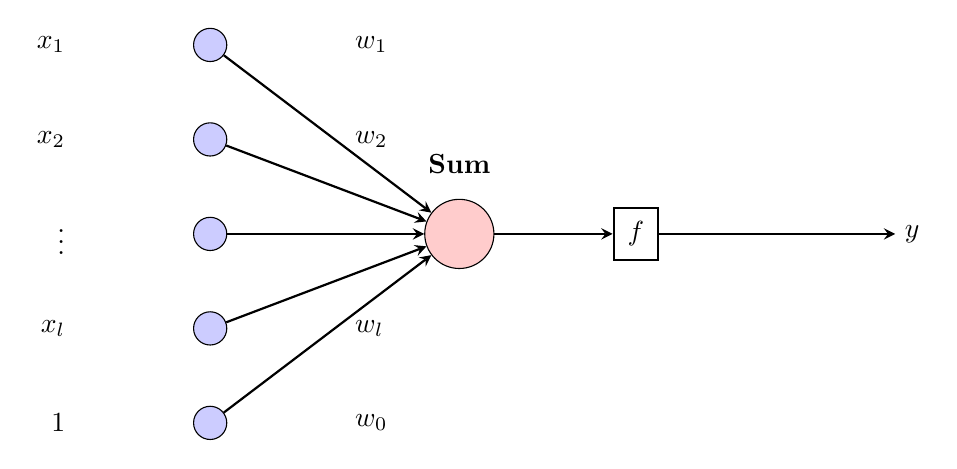
\begin{tikzpicture}[
        node distance=1.5cm,
        input neuron/.style={circle, draw, fill=blue!20, minimum size=12pt, inner sep=0pt},
        hidden neuron/.style={circle, draw, fill=red!20, minimum size=25pt, inner sep=0pt},
        block/.style={rectangle, draw, thick, minimum size=12pt, inner sep=5pt},
        output/.style={right of=block},
        neuron connection/.style={->, >=stealth, thick}
    ]

        % Input neurons
        \foreach \name/\label in {1/x_1, 2/x_2, 3/\vdots, 4/x_l, 5/1}
        {
            \node[input neuron] (I-\name) at (0,-\name*1.2) {};
            \node[left=of I-\name] {$\label$};
        }

        % Weights
        \foreach \name/\label in {1/w_1, 2/w_2, 4/w_l, 5/w_0}
        {
            \node[right=of I-\name] {$\label$};
        }

        % Neuron (hidden layer)
        \node[hidden neuron, right=2.5cm of I-3] (H-1) {};
        \node[above=0.2cm of H-1] {\textbf{Sum}};
        
        % Connections from inputs to neuron
        \foreach \i in {1,...,5}
        {
            \draw[neuron connection] (I-\i) -- (H-1);
        }

        % Activation function block
        \node[block, right=of H-1] (activation) {$f$};

        % Output y
        \node[output, right=of activation] (output) {$y$};

        % Connection from neuron to activation block and then to output
        \draw[neuron connection] (H-1) -- (activation);
        \draw[neuron connection] (activation) -- (output);

    \end{tikzpicture}
    \caption{A Perceptron Neuron with Activation Function Block}
    \label{fig:perceptron-neuron}
\end{figure}

A go-through of an input into a perceptron could be described as follows. 

\begin{equation}
    y = f(\mathbf{w}^\top\mathbf{x})
\end{equation}



\clearpage

\subsection{Perceptron Cost Function}
A \textbf{cost function} $\mathcal{J}(\mathbf{w})_{\delta_{\mathbf{x}}}$ is defined by the following:

\begin{equation}
    {\mathcal{J}(\mathbf{w})}_{\delta_{\mathbf{x}}} = 
        \sum_{\mathbf{x}\in\mathcal{X}_{\text{e}}}
        \delta_{\mathbf{x}}
        \mathbf{w}^\top \mathbf{x}
\end{equation}

where:

\begin{itemize}
    \item $\mathcal{X}_{\text{e}} \subset \mathcal{X}$ is a set of all wrongly-classified data samples. Surely, $\mathcal{X}_{\text{e}}$ is a subset of all the data samples $\mathcal{X}$.
    \item $\delta_{\mathbf{x}}$ is the cost, i.e., the punishment for this data sample to be different as the ground truth. In this section, we define it as follows: \\ $\delta_{\mathbf{x}}=\begin{cases}-1 & \text{if} \ \mathbf{x}\in\omega_1 \\ +1 & \text{if} \ \mathbf{x}\in\omega_2\end{cases}$
\end{itemize}

\begin{description}
    \item[Q:] Why is the cost function only accepting the parameter of $\mathbf{w}$?
    \item[A:] Because $\mathbf{x}$ are ground-truths that can't be changed. We are finding a hyperplane, i.e., a $\mathbf{w}$ that fits the unchanging $\mathbf{x}$.
\end{description}

The gradient of the cost function:

\begin{align}
    \dfrac
        {\partial {\mathcal{J}(\mathbf{w})}_{\delta_{\mathbf{x}}}}
        {\partial \mathbf{w}}
    &= 
    \dfrac
        {\partial}
        {\partial\mathbf{w}} 
    \sum_{x\in\mathcal{X}_{\text{e}}} 
    \delta_{\mathbf{x}} 
    \mathbf{w}^\top 
    \mathbf{x}
    \\
    &= 
    \sum_{\mathbf{x}\in\mathcal{X}_{\text{e}}}
    \delta_{\mathbf{x}}
    \mathbf{x} 
    \in \mathbb{R}^{l+1}
\end{align}

The gradient is a vector with the same shape as the weight vector $\mathbf{w}$, i.e., $l+1$. The gradient descent algorithm would be:

\begin{align}
    \mathbf{w}_{t+1} 
    &= 
        \mathbf{w}_{t} - 
        \gamma_{t} 
        \dfrac{\partial {\mathcal{J}(\mathbf{w})}_{\delta_{\mathbf{x}}}}
            {\partial \mathbf{w}}
        \Biggl|_{\mathbf{w}=\mathbf{w}_t}
    \\
    &= 
        \mathbf{w}_{t} -
        \gamma_{t}
        \sum_{\mathbf{x}\in\mathcal{X}_{\text{e}}}
        \delta_{\mathbf{x}}\mathbf{x}
\end{align}

where $\gamma_{t}$ is the learning rate at step $t$\footnote{
    The learning rate belongs to an explicit field of optimizers, which will not be discussed in this chapter. Just know that it is a scalar that changes every step.
}.


\end{document}